\chapter{Respuestas}
\label{chap:respuestas}
\section{IPv4}
\subsection{Muestra una captura de los 4 tipos paquetes DHCP intercambiados entre el nodo host[0] y el router durante el proceso de obtención de IP. Explica la función y la razón de las direcciones origen y destino de cada paquete.}

\begin{figure}[h]
    \centering
    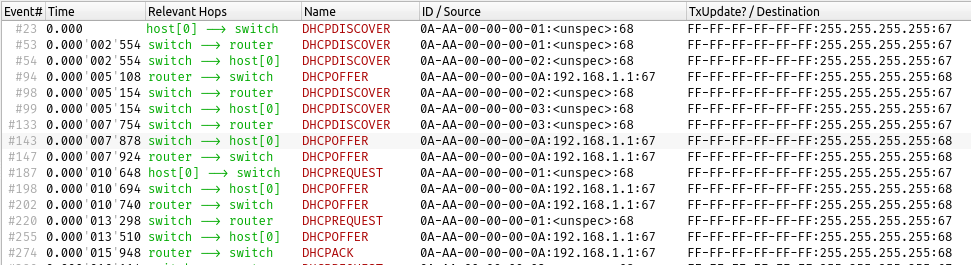
\includegraphics[width=\textwidth]{img/ej1.1.png}
    \caption{Paquetes DHCP entre host[0] y el router}
    \label{fig:ej1.1}
\end{figure}

 Como podemos ver en la figura \ref{fig:ej1.1}, los cuatros tipos de paquetes intercambiados son los siguientes:
 \begin{itemize}
     \item \textbf{DHCPDISCOVER:} Mensaje enviado por el cliente a la dirección \textit{broadcast} para buscar servidores DHCP disponibles y obtener una IP.\\ Tiene como dirección de origen la MAC del dispositivo emisor, la IP de origen sin especificar y, como destino, la MAC e IP de broadcast, ya que no conoce las direcciones del servidor (o los servidores) DHCP.
     \item \textbf{DHCPOFFER:} Mensaje enviado por un servidor DHCP como respuesta a un mensaje DHCPDISCOVER.\\ En este mensaje se envían al cliente los parámetros de configuración tales como la dirección IP que se le asignará, la subred, el tiempo de concesión de la dirección IP y la dirección IP del servidor DHCP que realiza la oferta.\\ Tienen la IP y MAC origen del router y como destino las MAC e IP de broadcast, ya que el cliente DHCP todavía no tiene IP asignada.
     \item \textbf{DHCPREQUEST:} Mensaje enviado por el cliente a la dirección \textit{broadcast}, en el que acepta la dirección IP ofrecida por el servidor DHCP que envió el mensaje DHCPOFFER y rechazando implícitamente ofertas realizadas por otros servidores DHCP.\\ Al igual que con DHCPDISCOVER, tiene la MAC del dispositivo emisor como origen, la IP de origen sin especificar (ya que todavía no tiene IP asignada) y como destino la MAC e IP de broadcast para que el paquete llegue a todos los servidores DHCP en la red.
     \item \textbf{DHCPACK:} Último mensaje en el proceso de configuración, enviado por el servidor DHCP. \\
     Con este mensaje se confirma la concesión de la dirección IP al cliente, y se le envían nuevamente los parámetros como la IP, la máscara y el tiempo de concesión. \\
     La IP y MAC de origen corresponden al router y las de destino corresponden a direcciones broadcast, debido a que el cliente sigue sin tener IP asignada.\\ 
     Una vez que el cliente reciba el mensaje, ya puede usar la IP asignada
 \end{itemize}

 
\subsection{¿De qué tipo son los primeros paquetes que se intercambian a partir de t = 6 segundos? ¿Cuál es su objetivo? ¿Cuáles son las direcciones origen y destino de estos paquetes (solicitud y respuesta)? ¿Tienen IP origen o destino? ¿Por qué?}
\begin{flushleft}
Los primeros paquetes emitidos en el instante \(t=6\) son del tipo ARP REQUEST y ARP REPLY, los cuales tienen como objetivo asociar una dirección IP con la MAC de un dispositivo.
El paquete ARP REQUEST es enviado por el cliente (host[1] en nuestro escenario) que quiere iniciar la nueva conexión TCP con el servidor en nuestra configuración y se utiliza para solicitar la dirección MAC de un dispositivo que está en nuestra red local. Este paquete tiene como dirección origen la dirección MAC del cliente (0A-AA-00-00-00-02) y como destino la dirección de Broadcast ethernet. Además, el contenido del paquete lo conforman la dirección IP y MAC del dispositivo origen (MAC: 0A-AA-00-00-00-02, IP: 192.168.1.3), y la dirección del servidor con el que se quiere establecer conexión en este caso (IP: 192.168.1.2, MAC:???). La dirección MAC destino se deja vacía ya que todavía es desconocida para el host de origen.
El paquete ARP REPLY lo envía el host al que pertenece la dirección IP destino que utilizamos en el ARP REQUEST (en nuestro caso el host[0]). Este paquete tiene como origen la MAC del servidor (0A-AA-00-00-00-01), como destino la MAC del cliente (0A-AA-00-00-00-02) y contiene las direcciones IP y MAC de origen y destino. Con este paquete, el servidor responde con su dirección MAC al dispositivo cliente que quería iniciar la conexión TCP. 
Estos paquetes no poseen dirección IP de origen ya el protocolo ARP es de la capa enlace, por lo que únicamente se utilizan las MACs de los dispositivos.
\end{flushleft}

\subsection{Elimina el cliente DHCP del host[3]. En su lugar, configúralo con una IP fija igual a la que el servidor DHCP asignará al host[0]. Para ello, añade una línea similar a la del router para el host[3] en el fichero config.xml. ¿Ocurre algún error cuando el host[0] recibe la IP ya asignada a host[3]? Describe qué ocurre durante el establecimiento de conexión TCP entre host[1] y host[0] a partir de t = 6 segundos.}
\begin{flushleft}\
Al asignar de manera estática la dirección 192.168.1.2 al host[3], no vemos ningún error en el momento en el que el router asigna dinámicamente la misma dirección al host[0]. Sin embargo, vemos que en \(t=6\), cuando el host[1] emite el ARP REQUEST para obtener la MAC del dispositivo que tiene asignada la IP 192.168.1.2, tanto host[0] como host [3] responden con un ARP REPLY. Cuando esto sucede, vemos en la simulación que el ARP REPLY de host[0] es el primero en llegar al cliente, iniciando la conexión TCP, pero acto seguido llega el ARP REPLY del host[3] y el cliente refresca su tabla ARP, dando como resultado que ahora host[3] es quién recibe todos los paquetes con destino 192.168.1.2. Como host[3] no tiene ningún servidor TCP corriendo, se entra en un bucle de RST y el cliente nunca logra iniciar conexión con el servidor. Este comportamiento se mantiene cada vez que host[1] refresca su tabla ARP.
\end{flushleft}
\section{IPv6}
\subsection{Asigna la misma MAC al host[3] y al host[0] y arranca la simulación. ¿Qué error ocurre antes de que haya transcurrido el primer segundo de simulación? ¿Qué paquete (tipo, origen y destino) provoca el error? ¿Por qué? Muestra una captura del error que aparece.}\label{1.2.1}
\begin{flushleft}
En nuestro escenario, configuramos la dirección MAC AA:AA:AA:AA:11:11 para el host[0] y host[3]. Al ejecutar la simulación, antes del primer segundo obtenemos un error indicando que existe una dirección link local duplicada en nuestra red local. Podemos ver este error en la captura \ref{fig:ej4.1}.

\begin{figure}[h]
    \centering
    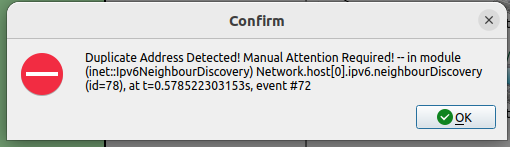
\includegraphics[width=\textwidth]{img/ej4.1.png}
    \caption{Error por direcciones IPv6 duplicadas}
    \label{fig:ej4.1}
\end{figure}

El error viene dado por un paquete de Neighbour Solicitation, ya que el host[3] envía un paquete cuyo destino es su propia dirección link-local y la MAC de broadcast, con el fin de detectar duplicados. Dado que el host[0] posee la misma dirección link-local, se detecta el error y se detiene la simulación.
\end{flushleft}


\subsection{Cambia la MAC del host[3] de manera que sólo difiera de la del host[0] en los primeros 3 bytes (es decir, el OUI). Mantén esta MAC para el resto de las preguntas. Muestra una captura del escenario en el momento inicial de la simulación en la que se vean las IPs link-local de los nodos host[*]. Explica cómo se construyen y los campos y bits destacables usando una dirección concreta como ejemplo. Utiliza para explicarlo la notación IPv6 no abreviada.}

\begin{figure}[h]
    \centering
    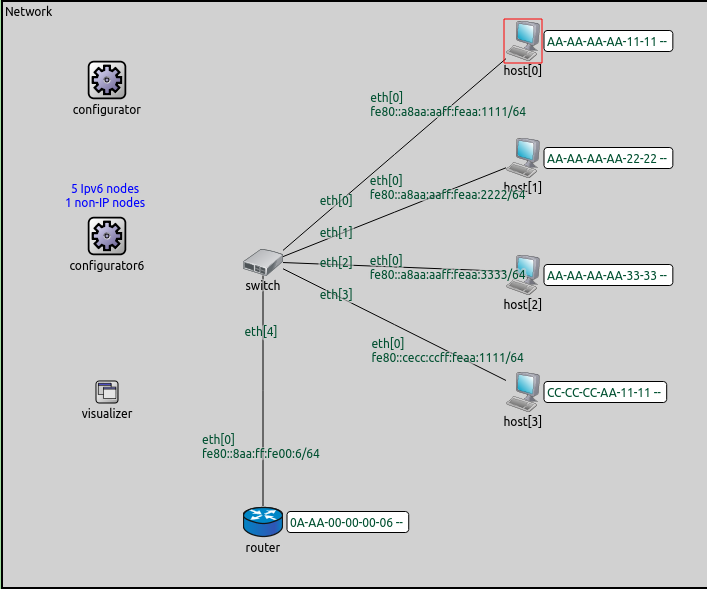
\includegraphics[width=\textwidth]{img/ej5.1.png}
    \caption{Escenario inicial}
    \label{fig:ej5.1}
\end{figure}

\begin{flushleft}
    Las direcciones link-local se generan automáticamente por el sistema operativo utilizando el prefijo de red fe80::/10, el cuál esta reservado para direcciones de enlace local. Los 54 bit siguientes (que indican la subred) se dejan a 0 en nuestro escenario, y los últimos 64 bits los conforma el ID de la interfaz. Este ID se puede configurar de tres maneras distintas:
\begin{itemize}
    \item \textbf{Manual:} Como su nombre indica, este ID se configura manualmente por el usuario.
    \item \textbf{Aleatorio:} El ID de red se configura con valores aleatorios.
    \item \textbf{EUI-64 IID:} El ID se crea a partir de los 48 bits de la MAC, insertando el valor hexadecimal 0xfffe (para completar los 64bits necesarios para el ID de interfaz) y por último cambiando el valor del séptimo bit (de izquierda a derecha), sustituyéndolo por su complemento.
\end{itemize}
En nuestra simulación, el ID de la interfaz se configura con EUI-64 IID, es por esto que si tomamos como ejemplo la MAC del host[1] (MAC: AA:AA:AA:AA:22:22), el ID de la interfaz pasa a ser A8AA:AAFF:FEAA:2222. Como resultado, obtenemos que la dirección IPv6 es FE80:0000:0000:0000:A8AA:AAFF:FEAA:2222. 
\end{flushleft}

\subsection{Muestra una captura del tráfico de paquetes en la que se vean las IP destino de los NS enviados desde cada uno de los nodos host[*] en los primeros 2 segundos. ¿Cuál es el motivo de esas IPs destino? ¿Como se construyen? ¿Coincide alguna de las IPs destino de los diferentes paquetes? ¿Por qué? ¿Qué consecuencia tiene esto?}

\begin{figure}[h]
    \centering
    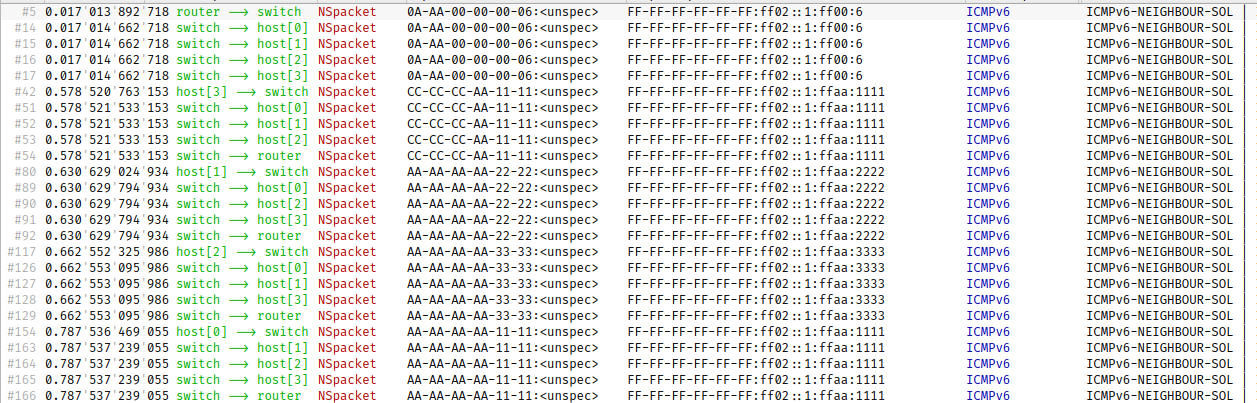
\includegraphics[width=\textwidth]{img/ej6.1.png}
    \caption{Paquetes NS en los primeros dos segundos}
    \label{fig:ej6.1}
\end{figure}
\begin{flushleft}
   Las direcciones IP destino que podemos ver en la captura \ref{fig:ej6.1} son direcciones multicast de nodo solicitado, y tienen como objetivo transmitir el paquete a dispositivos cuya MAC coincida con los últimos 24 bits de la dirección multicast. Estas IPs se forman utilizando el prefijo fe02::1:ff00:0000/104 y los últimos 24 bits de la dirección link-local asignada al host de origen.

En nuestra captura vemos que los paquetes enviados por host[0] y host[3] tienen como destino la misma dirección multicast. Esto se deben a que sus direcciones link-local coinciden en los 24 bits menos significativos (debido a las MACs configuradas en el escenario). La consecuencia de esto es que, cuando se emita el paquete proveniente de host[3], este va a ser aceptado por host[0] (ya que escucha su propia dirección mulicast de nodo solicitado), sin embargo, no responderá porque la dirección IPv6 contenida en el paquete no coincide con la link-local de host[0], por lo que no habrá ningún problema en la simulación y no saltará el error visto en la figura \ref{fig:ej4.1}. 
\end{flushleft}

\subsection{¿Qué MACs destino tienen los paquetes NS? ¿Cuáles deberían tener según lo visto en clases de teoría? (Utiliza uno de los paquetes NS como ejemplo y escribe los 6 bytes que debería tener la MAC en formato hexadecimal.) ¿Qué consecuencia tiene esta diferencia con respecto a lo visto en clase de teoría?}
\begin{flushleft}
    Tal y como vimos en la figura \ref{fig:ej6.1} , la dirección MAC de destino de los paquetes NS es FF-FF-FF-FF-FF-FF. Según lo visto en teoría, y si usamos el paquete NS emitido por host[0] (con MAC: AA-AA-AA-AA-11-11) como ejemplo, la MAC de destino debería ser la multicast 33-33-FF-AA-11-11, generada utilizando el prefijo 33-33 seguido de los 32 bits menos significativos de la MAC del dispositivo emisor. La consecuencia de no utilizar la dirección multicast, es que las tarjetas NIC no van a poder hacer el filtrado de paquetes según la MAC destino y tendrán que procesar los paquetes para determinar si deben ser descartados o no. Además, habrá un uso mayor del ancho de banda, ya que los paquetes NS van dirigidos a la MAC de broadcast y por ello se transmiten a todos los hosts en nuestra red.
\end{flushleft}


\subsection{¿En qué instante obtiene cada nodo host[*] su IP link-local definitiva (i.e., fin de DAD)? ¿En qué instante obtiene cada nodo su IP global? ¿Cómo obtienen esta última? Explica cómo se construye la IP global usando un nodo como ejemplo, de nuevo usando la notación IPv6 no abreviada. Muestra la tabla de interfaces de un nodo host en la que se vea su estado antes y después del DAD timeout, y antes y después de obtener la dirección global y explica qué cambia. (Nota: Qtenv muestra toda la información de cada interfaz en una línea; para verla correctamente copia el contenido con botón derecho → Copy Value y pégalo en la memoria como texto, en lugar de usar capturas de pantalla.)}
 \begin{flushleft}
     La dirección de enlace local definitiva se obtiene al momento de agotar el tiempo de espera para el DAD. Esto ocurre en los instantes:
\begin{itemize}
    \item host[3]: \(t=1.851\)
    \item host[1]: \(t=2.014\)
    \item host[2]: \(t=2.140\)
    \item host[0]: \(t=2.579\)
\end{itemize}. 
Los hosts obtienen su IP Global en el instante \(t= 2.826\), al momento de procesar el paquete de router advertisement que reciben. Esta dirección IP está formada por:
\begin{itemize}
    \item un prefijo de enrutamiento global que cubre los primeros 48 bits de la dirección IPv6.
    \item Un id de subred conformado por los siguientes 16 bits.
    \item El ID de la interfaz a la que se asocia esta dirección IP.
\end{itemize}

Si tomamos de ejemplo la dirección IPv6 link global del host[1] (IPv6 global aaaa:0005:0065:0000:a8aa:aaff:feaa:1111) tenemos que:
\begin{itemize}
    \item el prefijo de enrutamiento global es aaaa:0005:0065::/48
    \item El ID de subred es 0000.
    \item El ID de la interfaz (al igual que en la IPv6 de enlace local) es A8AA:AAFF:FEAA:2222.
\end{itemize}


\begin{lstlisting}[caption={Antes del DADTimeout y de obtener la dirección global}, label={list1}]
eth0 ID:101 MTU:1500 UP BROADCAST CARRIER MULTICAST macAddr:AA-AA-AA-AA-22-22 
 Ipv6:{
	Addrs:fe80::a8aa:aaff:feaa:2222(link tent)  expiryTime: inf prefExpiryTime: inf
	mcastgrps:ff02::1 	Node: dupAddrDetectTrans=1 reachableTime=40.327972322702
   }
\end{lstlisting}
\begin{lstlisting}[caption={Después del DADTimeout y antes de obtener la dirección global}, label={list2}]
eth0 ID:101 MTU:1500 UP BROADCAST CARRIER MULTICAST macAddr:AA-AA-AA-AA-22-22 
 Ipv6:{
	Addrs:fe80::a8aa:aaff:feaa:2222(link)  expiryTime: inf prefExpiryTime: inf
	mcastgrps:ff02::1 	Node: dupAddrDetectTrans=1 reachableTime=40.327972322702
   }
\end{lstlisting}

\begin{lstlisting}[caption={Después de obtener la dirección global}]
eth0 ID:101 MTU:1500 UP BROADCAST CARRIER MULTICAST macAddr:AA-AA-AA-AA-22-22 
 Ipv6:{
	Addrs:
     aaaa:5:65:0:a8aa:aaff:feaa:2222(global)  expiryTime: 2592002.826991341664 prefExpiryTime: 604802.826991341664,
     fe80::a8aa:aaff:feaa:2222(link)  expiryTime: inf prefExpiryTime: inf
	mcastgrps:ff02::1 	Node: dupAddrDetectTrans=1 reachableTime=3014.626181870699
   }
\end{lstlisting}

Como podemos ver en la tabla de interfaces \ref{list1}, antes de que termine el DAD tenemos que la dirección link local aparece como "link tent", lo que significa que está asignada tentativamente. Cuando DAD termina, la dirección de enlace local deja de ser tentativa y ahora la dirección contiene únicamente el texto "link". Por último, vemos que luego de que se asigna la dirección de enlace global nuestra interfaz eth0 pasa a tener dos direcciones, una global y la local anterior.
\end{flushleft}

\subsection{Muestra las IPs y MACs destino de los mensajes RS y RA que aparecen en torno al segundo 2 de simulación. ¿De qué tipo son estas IPs? ¿Por qué el RA no usa IP destino unicast? ¿Qué MACs destino deberían tener los RS y los RA según lo visto en clases de teoría?}
\begin{flushleft}
    \begin{figure}[h]
    \centering
    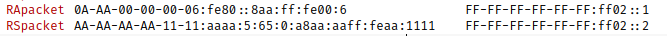
\includegraphics[width=\textwidth]{img/ej9.1.png}
    \caption{1º Columna: tipo de paquete. 2º Columna: Direcciones origen. 3º Columna: Direcciones destino.}
    \label{fig:ej9.1}
\end{figure}

En la figura \ref{fig:ej9.1} vemos que ambos paquetes utilizan direcciones IP multicast como destino. En el caso del paquete RA, se envía a la IP ff02::1 que indica que el paquete se emite para todos los dispositivos en la red local, mientras que la IP ff02::2 utilizada por RS indica que el paquete va dirigido para todos los routers. Los paquetes RA se emiten a una dirección multicast con el objetivo de enviar los parámetros de configuración a todos los dispositivos interesados en nuestra red local. Según la clase de teoría, las direcciones MAC que deben utilizarse para son la 33-33-00-00-00-01 para los paquetes RA y la MAC 33-33-00-00-00-02 para los paquetes RS. 

\end{flushleft}

\subsection{En t = 6 s se envía otro NS. ¿Para qué sirve? ¿Por qué es necesario? ¿Equivale a algún paquete en IPv4? Muestra una captura del log del nodo que lo envía que muestre el motivo del envío.}
\begin{flushleft}
    \begin{figure}[h]
    \centering
    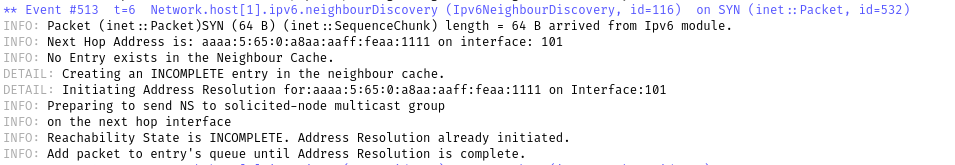
\includegraphics[width=\textwidth]{img/ej10.1.png}
    \caption{Evento en el que se muestra que no hay entrada en la Neighbour cache}
    \label{fig:ej10.1}
\end{figure}

En la figura \ref{fig:ej10.1} podemos ver que en el instante \(t = 6s\), host[1] intenta iniciar una conexión con host[0], sin embargo, en la neighbour cache no existe ninguna entrada con la IPv6 de destino, por lo que es necesario emitir un paquete NS con el objetivo de solicitar la MAC del dispositivo con el que se quiere establecer la conexión. Este paquete es el equivalente a emitir un paquete ARP REQUEST en IPv4.
\end{flushleft}

\subsection{¿De qué tipo es la IP destino de este paquete? Explica cómo se construye (notación IPv6 no abreviada). ¿Por qué no se usa una IP unicast para ese mensaje, si ya se conoce?}
\begin{flushleft}
    La dirección IP de destino es una dirección multicast de nodo solicitado. Esta dirección se construye de la siguiente manera:
\begin{itemize}
    \item Para los primeros 104 bits, se utiliza el prefijo fe02:0000:0000:0000:0000:0001:ff00:0000/104
    \item Para los últimos 24 bits, se utilizan los 24 bits menos significativos de la dirección IPv6 del dispositivo con el que se quiere establecer conexión, en nuestro caso, la dirección IPv6 del host[0] es aaaa:0005:0065:0000:a8aa:aaff:feaa:1111, por lo que los últimos 2 bits serán aa:1111
\end{itemize}
Con esto, tenemos que la dirección IPv6 destino del paquete NS es:

ff02:0000:0000:0000:0000:0001:ffaa:1111.

La razón por la que no utilizamos la IP unicast del servidor, es porque seguimos sin conocer su MAC, por lo que es necesario emitir un paquete a la dirección multicast y esperar a que el servidor responda con la MAC que le pertenece para poder establecer la conexión
\end{flushleft}


\subsection{¿En qué nodos host[*] llega este paquete NS al módulo ipv6? ¿Y al submódulo ipv6.neighbourDiscovery? ¿En qué nodos llegaría el mensaje al módulo ipv6 si INET implementase MACs multicast (33-33-xx-xx-xx-xx)? Razona las respuestas. (Nota: para ver el recorrido del paquete en el módulo ipv6, haz doble click en el nodo deseado y luego en el módulo ipv6. Puedes mostrar varios nodos a la vez en diferentes ventanas con botón derecho → Open Graphical View for ‘ipv6’ una vez dentro de ese nivel.)}
\begin{flushleft}
    El paquete NS llega al módulo ipv6 de todos los host excepto host[1] (ya que es quien lo emite), esto debido a que el paquete se envía a la MAC broadcast. Además, el paquete llega al submódulo ipv6.neighbourdiscovery de los host [0] y host[3], ya que la dirección multicast a la que se envía el paquete NS tiene como destinatarios estos dos host (aunque luego responda host[0] únicamente por tener asignada la IP por la que se pregunta).
    Si INET implementace MACs multicast, este paquete iría dirigido al host[0] y al host[3]. La razón es que al formarse la MAC multicast, daría como resultado 33-33-FF-AA-11-11, por lo que solo iría dirigido a los dispositivos cuya MAC coincida con los 24 bits menos significativos de la MAC multicast, siendo host[0] y host[3] los únicos que cumplen esta condición.
\end{flushleft}

\subsection{ Muestra capturas de la neighbour cache del nodo que envió el NS un segundo antes de enviarlo, justo después de enviarlo pero antes de recibir el paquete de respuesta y justo después de recibir la respuesta y explica las diferencias entre los 3 estados. (Nota: para ver la neighbour cache haz doble click sobre el nodo → ipv6 → neighbourDiscovery, y a continuación expande owned objects en la ventana inferior izquierda. La neighbour cache es el atributo neighbourMap.)}

\begin{figure}[h]
    \centering
    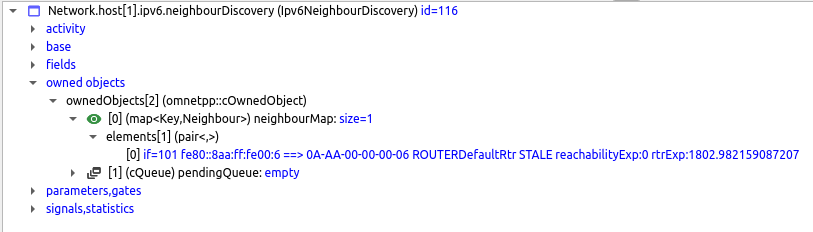
\includegraphics[width=1\textwidth]{img/ej13.1.png}
    \caption{Neighbour cache antes de emitirse el paquete NS}
    \label{fig:ej13.1}
\end{figure}

\begin{figure}[h]
    \centering
    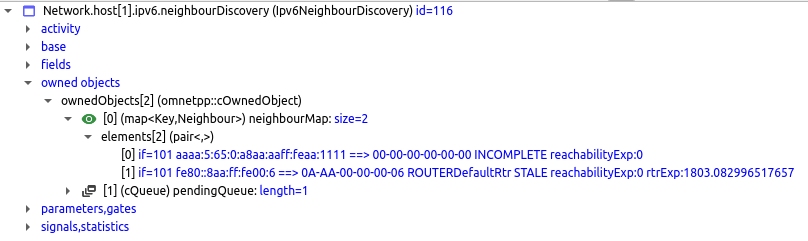
\includegraphics[width=1\textwidth]{img/ej13.2.png}
    \caption{Neighbour cache después de emitir el paquete NS y esperando respuesta}
    \label{fig:ej13.2}
\end{figure}

\begin{figure}[h]
    \centering
    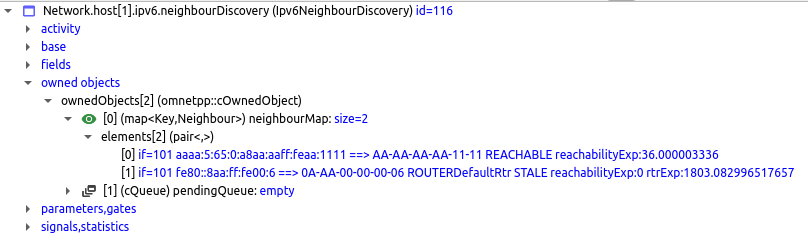
\includegraphics[width=1\textwidth]{img/ej13.3.png}
    \caption{Neighbour cache después de recibir respuesta al NS emitido}
    \label{fig:ej13.3}
\end{figure}
\begin{flushleft}
    Si comparamos las figuras \ref{fig:ej13.1} y \ref{fig:ej13.2}, vemos que la diferencia está en que, antes de emitir el paquete NS, la neighbour cache contenía una única entrada perteneciente a la dirección del Router. Una vez se envió el paquete, se añade a la cache una entrada incompleta y a la espera de una respuesta para completarse. Luego de que host[1] obtiene respuesta, vemos en la figura \ref{fig:ej13.3} que se completa la entrada con la MAC recibida como respuesta, añadiendo también un tiempo de expiración a la entrada.
\end{flushleft}

\subsection{¿Envía el host[1] algún otro mensaje NS después del instante t = 6 s? ¿Cuál es su objetivo? Muestra capturas del log en las que se muestre el motivo. ¿Es la IP destino de este NS del mismo tipo que en los NS enviados anteriormente? ¿Por qué?}

\begin{figure}[h]
    \centering
    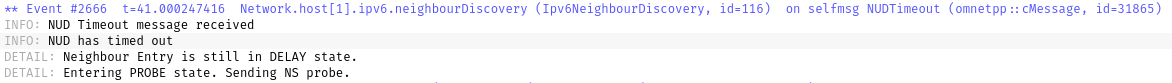
\includegraphics[width=\textwidth]{img/ej14.1.png}
    \caption{Paquete NS para refrescar la neighbour cache}
    \label{fig:ej14.1}
\end{figure}
\begin{flushleft}
    Si envía otro mensaje NS en \(t=6\), esto con el objetivo de refrescar la neighbour cache y verificar que la entrada siga siendo válida. Sin embargo, la dirección IP utilizada en este caso es la unicast del host[0]. Esto se debe a que la entrada ya existe en la neighbour cache, por lo que el paquete se puede dirigir a la IP y la MAC concreta del destinatario.
\end{flushleft}

\subsection{Muestra capturas de la neighbour cache del host[1] en los siguientes instantes de tiempo: 7 segundos antes del envío del NS de la pregunta anterior, 3 segundos antes del envío del NS, Justo después del envío del NS y antes de recibir el NA respuesta, Justo después de recibir el NA respuesta}

\begin{figure}[h]
    \centering
    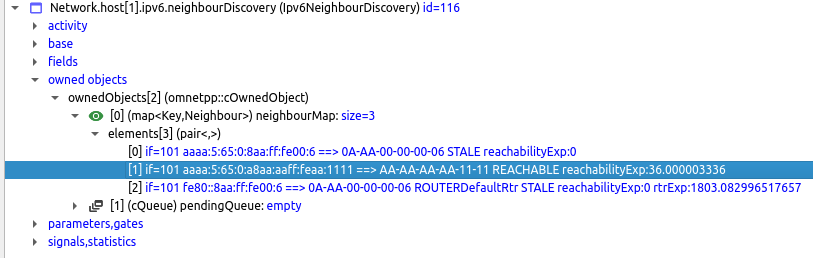
\includegraphics[width=\textwidth]{img/ej15.1.png}
    \caption{Neighbour cache 7s antes del envío del paquete NS}
    \label{fig:ej15.1}
\end{figure}

\begin{figure}[h]
    \centering
    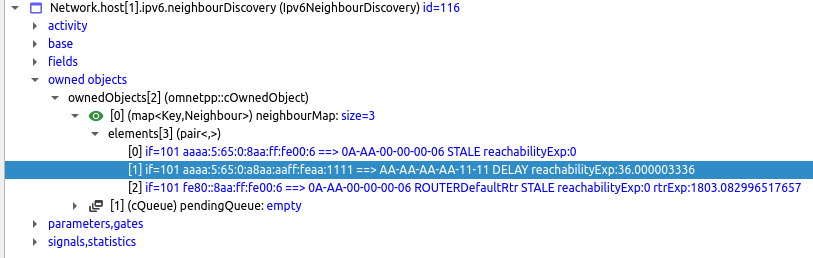
\includegraphics[width=\textwidth]{img/ej15.2.png}
    \caption{Neighbour cache 3s antes del envío del paquete NS}
    \label{fig:ej15.2}
\end{figure}

\begin{figure}[h]
    \centering
    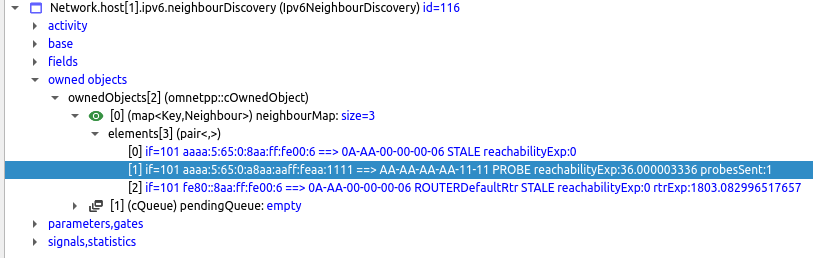
\includegraphics[width=\textwidth]{img/ej15.3.png}
    \caption{Neighbour cache justo después del envío del NS y antes de recibir el NA respuesta }
    \label{fig:ej15.3}
\end{figure}

\begin{figure}[h]
    \centering
    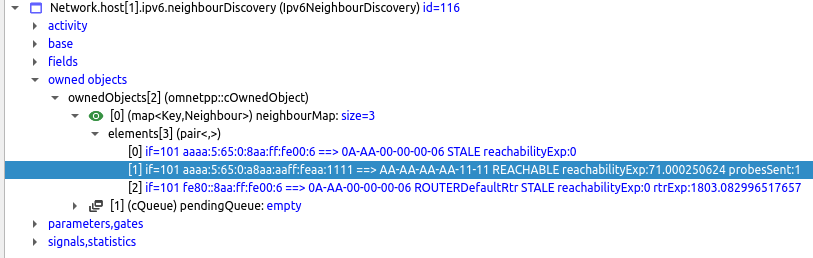
\includegraphics[width=\textwidth]{img/ej15.4.png}
    \caption{Justo después de recibir el NA respuesta }
    \label{fig:ej15.4}
\end{figure}
\begin{flushleft}
    Podemos apreciar en la figura \ref{fig:ej15.1} que, 7 segundos antes del envío del paquete NS, el nodo con IP aaaa:5:65:0:a8aa:aaff:feaa:1111 está en estado \textit{Reachable}, mientras que en la captura \ref{fig:ej15.2} observamos que 3s antes de emitirse el paquete, la entrada del mismo nodo pasó a estar en estado \textit{Delay}. Esto es debido a que se cumplió el tiempo de vencimiento de esta entrada. 
    Cuando llegamos al instante \(t= 41s\), vemos que se emite un paquete NS y vemos en la captura \ref{fig:ej15.3} la entrada de host[0] pasa a estar en estado \textit{Probe} en la neighbour cache, lo que implica que se esta intentando resolver la MAC nuevamente. Por último, vemos en la captura \ref{fig:ej15.4} 
\end{flushleft}
